\documentclass[12pt, letterpaper]{article}

\title{AA279c Project Report: Modeling the ISS}
\author{Toby J. Buckley}
\date{\today}




\usepackage{graphicx}
\usepackage{subcaption}
\usepackage{float}
\usepackage{amsmath}

\graphicspath{{./src/html/}}
\DeclareGraphicsExtensions{.pdf,.png,.jpg}

\begin{document}

\begin{titlepage}
	\maketitle
\end{titlepage}


testing



% 4 thrusters - 13.3 kg-f (29.3 lbf) https://www.quora.com/How-does-the-International-Space-Station-maintain-its-orbit-and-what-propellant-does-it-use



\section{Problem Set 4 - Gravity Gradient and Rotational Stability}


\begin{figure}[H]
	\centering
	\includegraphics[scale=0.9]{ps4_01}
	\caption{EKF performance.}
	\label{4:ekf}
\end{figure}


\begin{figure}[H]
	\centering
	\includegraphics[scale=0.9]{ps4_02}
	\caption{EKF performance.}
	\label{4:ekf}
\end{figure}


\begin{figure}[H]
	\centering
	\includegraphics[scale=0.9]{ps4_03}
	\caption{EKF performance.}
	\label{4:ekf}
\end{figure}


\begin{figure}[H]
	\centering
	\includegraphics[scale=0.9]{ps4_04}
	\caption{EKF performance.}
	\label{4:ekf}
\end{figure}


\begin{figure}[H]
	\centering
	\includegraphics[scale=0.9]{ps4_05}
	\caption{EKF performance.}
	\label{4:ekf}
\end{figure}


\begin{figure}[H]
	\centering
	\includegraphics[scale=0.9]{ps4_06}
	\caption{EKF performance.}
	\label{4:ekf}
\end{figure}


\begin{figure}[H]
	\centering
	\includegraphics[scale=0.9]{ps4_07}
	\caption{EKF performance.}
	\label{4:ekf}
\end{figure}






\section{Problem Set 5 - something}



\begin{figure}[H]
	\centering
	\includegraphics[scale=0.9]{ps5_01}
	\caption{EKF performance.}
	\label{5:ekf}
\end{figure}


\begin{figure}[H]
	\centering
	\includegraphics[scale=0.9]{ps5_02}
	\caption{EKF performance.}
	\label{5:ekf}
\end{figure}


\begin{figure}[H]
	\centering
	\includegraphics[scale=0.9]{ps5_03}
	\caption{EKF performance.}
	\label{5:ekf}
\end{figure}


\begin{figure}[H]
	\centering
	\includegraphics[scale=0.9]{ps5_04}
	\caption{EKF performance.}
	\label{5:ekf}
\end{figure}


\begin{figure}[H]
	\centering
	\includegraphics[scale=0.9]{ps5_05}
	\caption{EKF performance.}
	\label{5:ekf}
\end{figure}


\begin{figure}[H]
	\centering
	\includegraphics[scale=0.9]{ps5_06}
	\caption{EKF performance.}
	\label{5:ekf}
\end{figure}


\begin{figure}[H]
	\centering
	\includegraphics[scale=0.9]{ps5_07}
	\caption{EKF performance.}
	\label{5:ekf}
\end{figure}

\section{Problem Set 6 - Attitude Determination with Sensor Errors}



\begin{figure}[H]
	\centering
	\includegraphics[scale=0.9]{ps6_01}
	\caption{EKF performance.}
	\label{6:ekf}
\end{figure}


\begin{figure}[H]
	\centering
	\includegraphics[scale=0.9]{ps6_02}
	\caption{EKF performance.}
	\label{6:ekf}
\end{figure}


\begin{figure}[H]
	\centering
	\includegraphics[scale=0.9]{ps6_03}
	\caption{EKF performance.}
	\label{6:ekf}
\end{figure}


\begin{figure}[H]
	\centering
	\includegraphics[scale=0.9]{ps6_04}
	\caption{EKF performance.}
	\label{6:ekf}
\end{figure}


\begin{figure}[H]
	\centering
	\includegraphics[scale=0.9]{ps6_05}
	\caption{EKF performance.}
	\label{6:ekf}
\end{figure}


\begin{figure}[H]
	\centering
	\includegraphics[scale=0.9]{ps6_06}
	\caption{EKF performance.}
	\label{6:ekf}
\end{figure}




\section{Problem Set 7 - Implement Extended Kalman Filter}



\begin{figure}[H]
	\centering
	\includegraphics[scale=0.9]{ps7_01}
	\caption{EKF performance.}
	\label{7:ekf}
\end{figure}


\begin{figure}[H]
	\centering
	\includegraphics[scale=0.9]{ps7_02}
	\caption{EKF performance.}
	\label{7:ekf}
\end{figure}


\begin{figure}[H]
	\centering
	\includegraphics[scale=0.9]{ps7_03}
	\caption{EKF performance.}
	\label{7:ekf}
\end{figure}


\begin{figure}[H]
	\centering
	\includegraphics[scale=0.9]{ps7_04}
	\caption{EKF performance.}
	\label{7:ekf}
\end{figure}


\begin{figure}[H]
	\centering
	\includegraphics[scale=0.9]{ps7_05}
	\caption{EKF performance.}
	\label{7:ekf}
\end{figure}


\begin{figure}[H]
	\centering
	\includegraphics[scale=0.9]{ps7_06}
	\caption{EKF performance.}
	\label{7:ekf}
\end{figure}



\section{Problem Set 8 - Implement Actuators and Controllers}

The International Space Station uses 4 control-moment-gyros it uses for day-to-day station keeping. Each CMG can produce 4760 N*m*s, or 258 N*m, and spins at 691 rad/s. In reality, the ISS has all four aligned the in the same direction, but for simplicity I've decided to model three CMG's each aligned in a different body axis direction.

The control moment gyros operate by running at a fixed very high speed rotation, with large mass and radius. By gimbaling the CMG, the angular momentum vector is shifted which causes a reaction torque on the rest of the satellite due to the conservation of angular momentum.


\begin{equation}
I\dot{\omega} + \omega x I\omega = M + M_c;\ M_c = -A\dot{L_w}-\dot{A}L_w-\omega x AL_w
\label{8:eq1}
\end{equation}

Because we have changed the dynamics of the vehicle by adding additional large rotating masses, the Euler equations must also change. Eq. \ref{8:eq1} shows how the CMG's are taken into account, by grouping them together into a control moment term, which we are able to take advantage of when determining a control sequence. 

Control of the aircraft is performed using two successive loops (Fig. \ref{8:controller}). First, a high-level objective attitude is created (example: follow the RTN frame) and passed to the attitude controller. A first controller generates commanded angular velocity, which is passed to the second controller. The output of the inner-loop are the desired moments that the CMG's must impart on the vehicle. Those are perturbed slightly by assuming imperfect actuators, and then passed into the environment simulator. The required CMG angles are computed from the control-loop output by solving for $\dot{A}$ and performing a 1st order integration.


\begin{figure}[H]
	\centering
	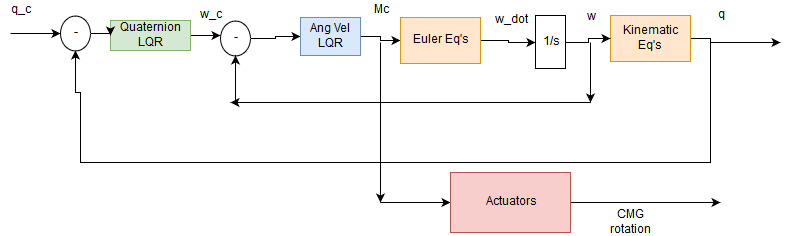
\includegraphics[scale=0.7]{PS8_controller}
	\caption{Block diagram for the controller used onboard the satellite. Two LQR's are utilized, one for attitude and the other for a lower-level ang. vel. controller.}
	\label{8:controller}
\end{figure}

The block diagram for the controller (Fig. \ref{8:controller}) shows how the different controllers pass information to each-other and the environment. In order to obtain the controller gains, a linear-quadratic controller is implemented.

\begin{gather}
x_{k+1}=Ax_k+Bu_k
\label{8:discrete} \\ 
u=-Kx
\label{8:lqr}
\end{gather}

The linear-quadratic controller, or LQR, is well-documented and used widely in the controls community. Eq. \ref{8:discrete} shows the discrete state space model, where the next state is a linear function of the current state and controls. It's assumed a linear gain is applied to the state and used to control the system (Eq. \ref{8:lqr}). By setting a weight matrix for the state ($Q$), for the control ($R$), and for the combination state and control ($N$), an optimal gain matrix can be solved for which minimizes the cost of regulating the system (shown below). The matlab function $K=dlqr(A,B,Q,R)$ is used to obtain the gain matrix.

\begin{figure}[H]
	\centering
	\includegraphics[scale=0.7]{ps8_lqrCost}
	\label{8:lqrCost}
\end{figure}


The plant matrix, $A$, was obtained by linearizing the euler and kinematic equations. Taylor series expansion (shown below) was used to obtain a first order approximation of the differential equations.

\begin{figure}[H]
	\centering
	\includegraphics[scale=0.7]{ps8_taylor}
	\label{8:taylor}
\end{figure}

For attitude, $\dot{q} = 1/2\Omega q$ was linearized with respect to angular velocity. Below is the jacobian of $q$, as well as the discrete next-step quaternion.

\[
\nabla_\omega q =
\begin{bmatrix}
q4 &-q3 &q2 \\
q3 &q4 &-q1 \\
-q2 &q1 &q4 \\
-q1 &-q2 &-q3
\end{bmatrix}
;\ q_{k+1} \approx dt*1/2*\nabla_\omega q|_q*\omega + q_k
\]

Eq. \ref{8:discreteQuat} places the known quantities into the usual discrete linear system form. For the inner-loop, the same linear model used in the EKF is used here.

\begin{equation}
q_{k+1} = A q_k + B \omega;\ A = eye(4),\ B = dt*1/2*\nabla_\omega q|_q
\label{8:discreteQuat}
\end{equation}

In the simulink model, the control loop is ran once every ten time-steps. This is valid because linearized dynamics are accurate within an area surrounding the point of linearization. Satellite's dynamics evolve relatively slow compared to the time-step, so the gain matrix is only updated sparingly.

Initially, I had significant trouble getting the LQR controllers to function properly. The satellite could control its ang. vel., but not the attitude. After careful inspection, I figured out the issue: the weight matrices on each LQR were not properly adjusted after implementing the successive control-loop structure. With no feed-forward terms or direct coupling between attitude and control moment, there is a natural delay whenever an attitude is commanded. If the attitude controller doesn't allow enough time for the ang. vel. to 'catch up', then it will change the commanded ang. vel. before anything even happens. This was resolved by weighting the attitude rather low, and the ang. vel. higher, so that the inner-loop reaches the commanded velocity much quicker and is able to affect the attitude as desired.

In testing the controller, a nominal trajectory was defined for the ISS to follow. The satellite begins in the RTN frame with $\omega=[0 -n0 0]'$ and is subject to perturbations. The goal is to maintain the desired attitude.

\begin{figure}[H]
	\centering
	\includegraphics[scale=0.9]{ps8_01}
	\caption{Angular velocity with and without control.}
	\label{8:angvel}
\end{figure}

Fig. \ref{8:angvel} shows how the euler angles evolve during the flight. With no control the yaw and pitch vary sinusoidally due to the perturbations present. With active control the euler angles converge onto their nominal value and retain them for the rest of the flight. The jitter in the beginning is due to the EKF's random initialization. It hasn't yet converged onto the true value so when $\omega_{measured}$ is fed into the controller it produces garbage control moments.

\begin{figure}[H]
	\centering
	\includegraphics[scale=0.9]{ps8_02}
	\caption{EKF performance.}
	\label{8:ekf}
\end{figure}

Fig. \ref{8:ekf} shows how the extended kalman filter behaves near the beginning of the flight. After randomly initializing the state, new observations allow the EKF to quickly determine the optimal $P$ matrix and converge onto the true observations. Within 10 seconds, the error in angular velocity approaches zero.

\begin{figure}[H]
	\centering
	\includegraphics[scale=0.9]{ps8_03}
	\caption{Error in attitude control between principle and RTN frames.}
	\label{8:attError}
\end{figure}

Above is the attitude control error during the flight. This represents the direction cosine matrix between principle axes and RTN frame. Perturbations and state uncertainty lead to some drift between the frames, but the active controller quickly overcomes them and returns the ISS to its nominal attitude.

\begin{figure}[H]
	\centering
	\includegraphics[scale=0.9]{ps8_04}
	\caption{Angular velocity while de-tumbling.}
	\label{8:angvel}
\end{figure}

The output of the controller is how much moment to impart in each principle direction. Besides the initial jitter, very little moment is required to keep the orbit.

\begin{figure}[H]
	\centering
	\includegraphics[scale=0.9]{ps8_05}
	\caption{Angular velocity while de-tumbling.}
	\label{8:angvel}
\end{figure}

After control moments are generated, the amount of gimbal required to provide them is calculated. Above shows how the combined CMG system must rotate in order to satisfy the controller's requirements. This result is troubling, as each CMG needs to rotate multiple revolutions to keep the station for part of an orbit. I suspect a bug or a sizing issue.



\section{Problem Set 9 - Define and Execute a Slew Maneuver}
A problem all satellites deal with is de-tumbling. When launched into orbit the satellite is harshly ejected from its rocket into a target orbit and must immediately begin to align itself into its nominal position. I've simulated a tumbling environment by setting $w0=rand(3,1)$ and allowing the dynamics and controller to stabilize the system naturally. The target attitude for the de-tumble is the earth-facing RTN frame.


\begin{figure}[H]
	\centering
	\includegraphics[scale=0.9]{ps9_01}
	\caption{Angular velocity while de-tumbling.}
	\label{9:angvel}
\end{figure}

Fig. \ref{9:angvel} shows the angular velocity while de-tumbling. Because of the high priority on matching $w$ to $w_{desired}$ the velocities stabilize quickly. After that all changes are due to the attitude controller commanding certain angular velocity in order to align itself with the RTN frame.


\begin{figure}[H]
	\centering
	\begin{subfigure}[b]{0.49\textwidth}
	\includegraphics[width=\textwidth]{ps9_02}
	\end{subfigure}
	\begin{subfigure}[b]{0.49\textwidth}
		\includegraphics[width=\textwidth]{ps9_03}
	\end{subfigure}
	\caption{The position during a de-tumble. The Target is earth-facing in the RTN frame.}
	\label{(9:pos)}
\end{figure}

Fig. \ref{(9:pos)} shows how the principle axes aligns itself with the RTN frame over time. Oscillations are present due to the sinusoidal dynamics of the rotation cosine matrices.

\begin{figure}[H]
	\centering
	\includegraphics[scale=0.9]{ps9_04}
	\caption{Attitude control error until convergence.}
	\label{9:atterror}
\end{figure}

Fig \ref{9:atterror} shows the evolution of the attitude control error over time. It's clear the the tumbling has a huge effect on the relative alignment of the principle axes with the desired RTN frame. But this problem is overcome within 800 seconds of ejection with the satellite's onboard controller.




\end{document}